\documentclass{article}

% to avoid loading the natbib package, add option nonatbib:
% \usepackage[nonatbib]{style}

\usepackage[final]{style}
\usepackage{graphicx}
\usepackage[utf8]{inputenc} % allow utf-8 input
\usepackage[T1]{fontenc}    % use 8-bit T1 fonts
\usepackage{hyperref}       % hyperlinks
\usepackage{url}            % simple URL typesetting
\usepackage{booktabs}       % professional-quality tables
\usepackage{amsfonts}       % blackboard math symbols
\usepackage{nicefrac}       % compact symbols for 1/2, etc.
\usepackage{microtype}      % microtypography
\usepackage{verbatim}
\usepackage{cite}
\usepackage{float}


\title{Formatting instructions for VC36O Notes}

% The \author macro works with any number of authors. There are two
% commands used to separate the names and addresses of multiple
% authors: \And and \AND.
%
% Using \And between authors leaves it to LaTeX to determine where to
% break the lines. Using \AND forces a line break at that point. So,
% if LaTeX puts 3 of 4 authors names on the first line, and the last
% on the second line, try using \AND instead of \And before the third
% author name.

\author{
  Elaine C. Sangali, Douglas Abreu \\
  Department of Computer Science\\
  Federal University of Technology - Paran\'{a} / UTFPR\\
  Campo Mour\~{a}o, Paran\'{a}, Brazil \\
  \texttt{\{e.nani92, douglasabrel97\}@gmail.com} \\
  %% examples of more authors
  %% \And
  %% Coauthor \\
  %% Affiliation \\
  %% Address \\
  %% \texttt{email} \\
  %% \AND
  %% Coauthor \\
  %% Affiliation \\
  %% Address \\
  %% \texttt{email} \\
  %% \And
  %% Coauthor \\
  %% Affiliation \\
  %% Address \\
  %% \texttt{email} \\
  %% \And
  %% Coauthor \\
  %% Affiliation \\
  %% Address \\
  %% \texttt{email} \\
}

\begin{document}

\maketitle

\section{Introdução a Visão Computacional}
    De acordo com \citeonline{cavalca} e \citeonline{marengoni}, o olho e o cérebro humano conseguem fazer o reconhecimento de objetos e detectar padrões em imagens muito bem, e muitos tentam replicar isso para um modelo computacional.
    
    A visão computacional procura replicar a visão humana, tentando reconhecer objetos, organizar informações, montar objetos e detectar padrões em imagens. Tanto na visão computacional quanto no processamento de imagens, a entrada é uma imagem, mas no processamento de imagens a saída pode ser um conjunto de valores numéricos, que podem ou não compor uma outra imagem, já na visão computacional a saída é uma interpretação da imagem como um todo, ou parcialmente.
    
    Um dos maiores desafios da visão computacional é detectar padrões em uma imagem, para isso é necessário que a imagem passe por alguns processamentos, como a remoção de ruídos através da filtragem, assim alguns algoritmos podem ser executados para conseguir separar e identificar os objetos da imagem como mostra a figura \ref{fig:fig1}.
    
     \begin{figure}[H]
        \centering
        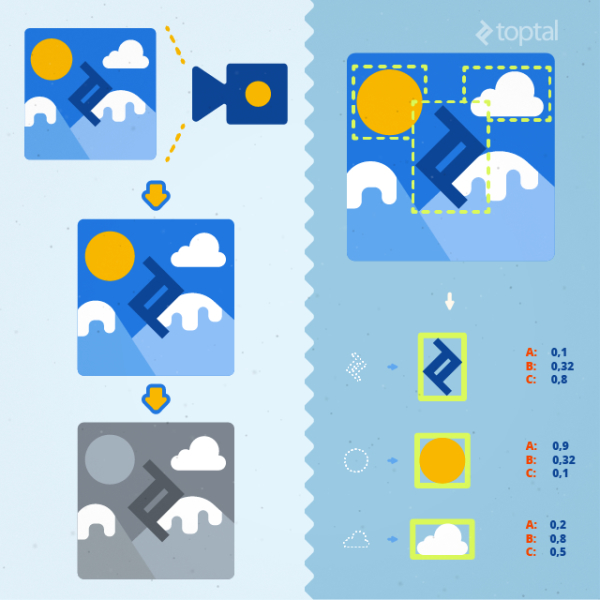
\includegraphics[width=0.6\textwidth]{template/img/fig1.jpg}
        \caption{Exemplo de detecção de padrões em uma imagem.}
        \label{fig:fig1}
    \end{figure}
    
    \subsection{Aplicações}

    Uma das aplicações da visão computacional é a medicina, onde é realizado a extração das informações das imagens afim de realizar diagnósticos sobre os pacientes, como exemplo, as imagens de microscopia, de radiografia, de angioplastia, de ultrassonografia, de tomografia e de Ressonância magnética.
    
    A visão computacional também é utilizada para outras aplicações, como aplicações militares onde é feito a detecção de unidades inimigas ou mísseis tele-guiados.
    
    Uma aplicação que está chamando a atenção ultimamente são os veículos autônomos, onde utilizam visão computacional para a navegação, para detectar obstáculos, manter o carro na pista, obter a localização e produzir mapas do ambiente.

    \subsection{Processos}
    
    Segundo a \citeonline{wikipedia} alguns dos processos utilizados na visão computacional são:
    
     \begin{quotation}
     
    \textbf{Aquisição de imagem:} uma imagem digital é produzida por um ou vários sensores. Dependendo do tipo do sensor, o resultado pode variar entre uma imagem bidimensional, uma cena tridimensional ou ainda uma sequência de imagens. Os valores dos pixels geralmente indicam a intensidade da luz em uma ou várias faixas de cor (o que forma imagens em tom de cinza ou coloridas), mas também podem indicar valores físicos como profundidade e absorção ou reflexão das ondas eletromagnéticas.
    
    \textbf{Pré-processamento:} antes de um método de visão computacional ser aplicado em uma imagem para extrair informação, é geralmente necessário processar a imagem para assegurar-se que ela satisfaz as condições do método. Exemplos incluem remapeamento (para assegurar o sistema de coordenadas), redução de ruídos (para assegurar que as informações são verdadeiras) e aumento de contraste (para assegurar que as informações relevantes serão detectadas).
    
    \textbf{Extração de características:} características matemáticas da imagem em vários níveis de complexidade são extraídos. Exemplos básicos incluem detecção de bordas, cantos ou pontos. Exemplo sofisticados incluem a morfologia matemática, detecção de texturas, formatos e movimentos.
    
    \textbf{Detecção e segmentação:} em algum ponto do processo uma decisão é feita sobre a relevância de regiões da imagem para processamento posterior. Exemplos incluem a seleção de regiões de interesse específicos e segmentação de uma ou mais regiões que contém um objeto de interesse.
    
    \textbf{Processamento de alto nível:} neste ponto a entrada é geralmente um conjunto pequeno de dados. O processo posterior inclui a verificação da satisfação dos dados, a estimativa de parâmetros sobre a imagem e a classificação dos objetos detectados em diferentes categorias.

 \end{quotation}
    
\section{Representação de imagens}
    Para \citeonline{cavalcanti}, as imagens são formadas por primitivas gráficas, tendo elas cores ou não. As primitivas gráficas são os elementos básicos que formam um desenho, como exemplo o ponto, segmento, polilinha, polígono, arco de elipse, etc.
    
    As imagens podem ser do tipo vetorial ou matricial, as imagens do tipo vetorial são formadas através de primitivas gráficas, por exemplo, para desenhar uma girafa o desenho não será feito por pixel como o matricial, será utilizado quadrados, linhas, círculos, etc, como mostra a figura \ref{fig:fig2}.
    
     \begin{figure}[H]
        \centering
        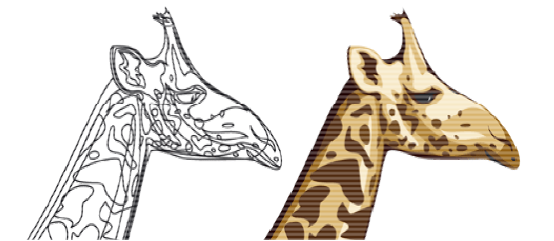
\includegraphics[width=0.6\textwidth]{template/img/fig2.png}
        \caption{Exemplo de imagem vetorial.}
        \label{fig:fig2}
    \end{figure}
    
    Na representação matricial, a imagem é formada por uma matriz onde cada quadrado representa um pixel. Os objetos são formados através do preenchimento desses pixeis afim de formar um desenho. As imagens matriciais também são conhecidas como bitmaps. Na figura \ref{fig:fig3} podemos ver como a imagem é formada.
    
    \begin{figure}[H]
        \centering
        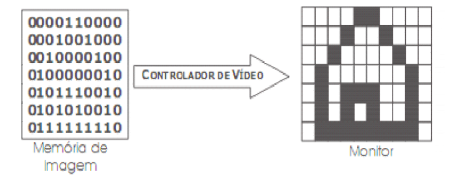
\includegraphics[width=0.6\textwidth]{template/img/fig3.png}
        \caption{Exemplo de imagem matricial.}
        \label{fig:fig3}
    \end{figure}
    
    Através da figura \ref{fig:fig4} podemos ver a diferença entre a representação vetorial e matricial.
    
    \begin{figure}[H]
        \centering
        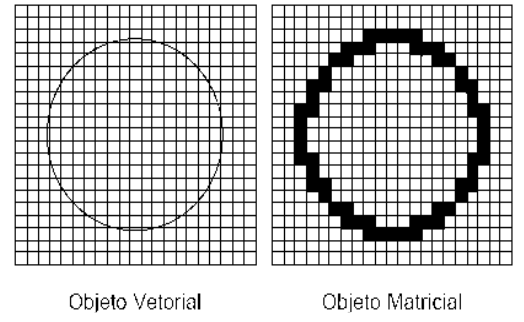
\includegraphics[width=0.6\textwidth]{template/img/fig4.png}
        \caption{Imagem vetorial vs Imagem matricial.}
        \label{fig:fig4}
    \end{figure}
    
\section{Filtragem de imagens}
     O \citeonline{demisio}, explica que a filtragem é utilizada para melhorar a qualidade das imagens através da ampliação do seu contraste, eliminação  de  padrões  periódicos  ou aleatórios, melhoria  no  seu  foco  e  acentuação  de características. As técnicas de filtragem são transformações da imagem pixel a pixel, que não dependem apenas do nível de cinza de um determinado pixel, mas também do valor dos níveis de cinza dos pixeis vizinhos. Afim de melhorar a imagem é feito uma multiplicação com a matriz da imagem atual com a máscara do filtro escolhido.
    
    Analisando as imagens  podemos  encontrar as frequências altas e baixas. Sendo assim possível  reduzir  os  efeitos  de determinadas  frequências  na imagem,  buscando obter  um  efeito  visual  de  melhor  qualidade  na  imagem.  
    
    \subsection{Filtros passa baixas}
    Os  filtros Passa  Baixas  eliminam os ruídos causados por altas frequências em imagens. As altas frequências podem causar uma  desfocalização caracterizada  por  uma  imagem borrada.
    
    Exemplos de filtros passa baixa:
     
    \textbf{Filtro da Média:} O pixel central é a média aritmética dos pixeis dentro da área da janela. De acordo com a figura as máscaras utilizadas são:
    
    \begin{figure}[H]
        \centering
        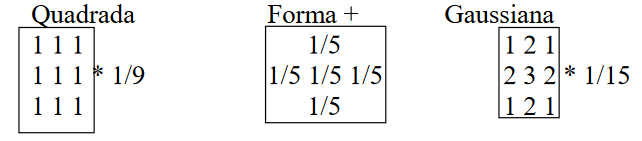
\includegraphics[width=0.6\textwidth]{template/img/fig5.png}
        \caption{Máscara dos filtros da média.}
        \label{fig:fig5}
    \end{figure}
    
    \textbf{Filtro da Média Ponderada:} O peso depende de sua distância ao peso central. Neste  caso  a  suavização  é  menos  intensa  pois  há  mais  influência  do pixel central.  
    
    \begin{figure}[H]
        \centering
        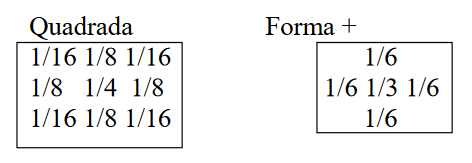
\includegraphics[width=0.5\textwidth]{template/img/fig6.png}
        \caption{Filtro da média ponderada.}
        \label{fig:fig6}
    \end{figure}
    
    \textbf{Filtro da Moda:} O nível de cinza do pixel central é o nível de cinza mais populoso dentro da janela de dimensão do filtro. Este  filtro  é  usado  para  homogeneizar  imagens  temáticas,  ou  para  reduzir ruídos mantendo o máximo de informação na imagem. 
    
     \begin{figure}[H]
        \centering
        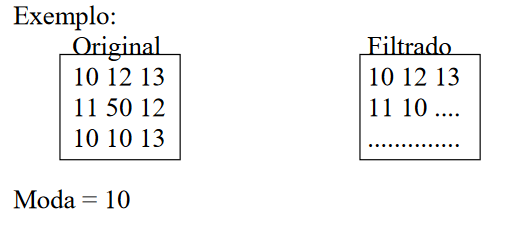
\includegraphics[width=0.5\textwidth]{template/img/fig7.png}
        \caption{Filtro da moda.}
        \label{fig:fig7}
    \end{figure}
    
    \textbf{Filtro  da  Mediana:} O  nível  de  cinza  do  pixel  central  é  o  nível  de cinza  intermediário  do  conjunto  ordenado  de  níveis  de  cinza  dentro  da janela. Este  é  um  filtro  complexo  por  envolver  ordenação.  Mas  sua aplicação suaviza a imagem preservando a informação de bordas na imagem. 
    
    \begin{figure}[H]
        \centering
        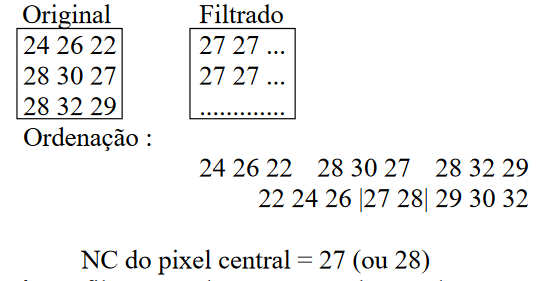
\includegraphics[width=0.6\textwidth]{template/img/fig8.png}
        \caption{Filtro da mediana.}
        \label{fig:fig8}
    \end{figure}
    
    \subsection{Filtro passa alta}
    
    Os Filtros  Passa  Altas  (FPA)  ou  de  realce  de  bordas, são usados para realçar os detalhes em uma imagem, atenuando  ou  eliminando  as  baixas  frequências,  realçando  assim as altas frequências. O   tamanho   da   máscara   (filtro)   utilizado   influencia   o   resultado  final.  Quanto  menor  forem  as  dimensões  do  filtro,  menos  detalhes  serão  realçados.  No  caso  de  feições  lineares  extensas,  usa-se  máscaras de dimensões grandes. 
    
    Filtros Laplacianos : usados para detectar bordas. Estas máscaras caracterizam-se por ter a soma dos pesos = 0.
    
     \begin{figure}[H]
        \centering
        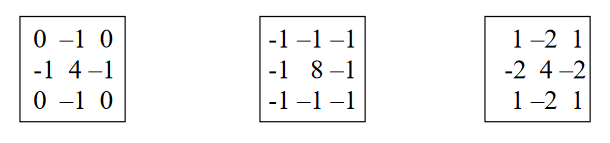
\includegraphics[width=0.6\textwidth]{template/img/fig9.png}
        \caption{Filtro Laplacianos.}
        \label{fig:fig9}
    \end{figure}
    
    Para entender melhor a diferença entre o filtro passa baixa e alta, considere as figuras \ref{fig:fig19}, \ref{fig:fig20} e \ref{fig:fig21} .
    
    \begin{figure}[H]
        \centering
        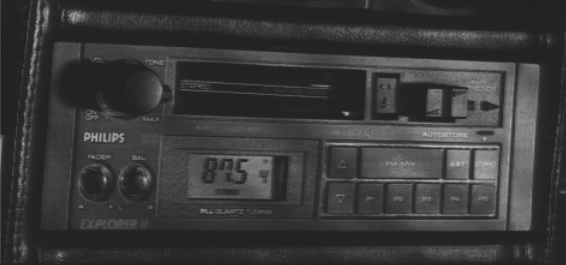
\includegraphics[width=0.6\textwidth]{template/img/fig19.png}
        \caption{Imagem original.}
        \label{fig:fig19}
    \end{figure}
    
    \begin{figure}[H]
        \centering
        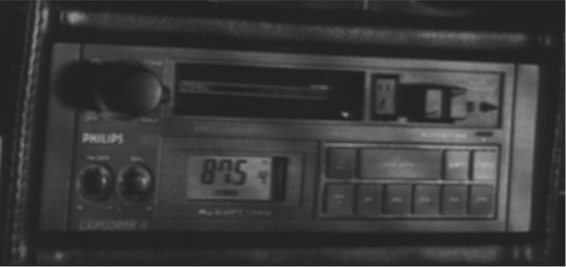
\includegraphics[width=0.6\textwidth]{template/img/fig20.png}
        \caption{Aplicado o filtro passa baixa.}
        \label{fig:fig20}
    \end{figure}
    
    \begin{figure}[H]
        \centering
        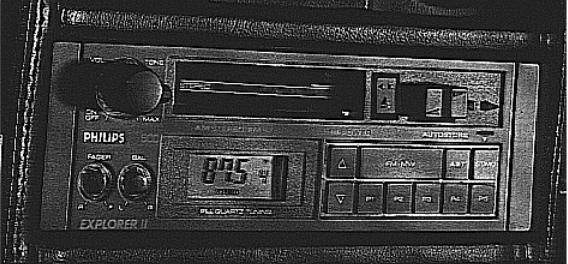
\includegraphics[width=0.6\textwidth]{template/img/fig21.png}
        \caption{Aplicado o filtro passa alta.}
        \label{fig:fig21}
    \end{figure}
    
    

\section{Correlação}
    Correlação são operações básicas para extrair informações de uma imagem.
    
    
\subsection{Exemplo}
    Vamos considerar uma simples operação de média, na qual substituímos cada pixel em uma imagem 1D pela média de esse pixel e seus dois vizinhos. Suponha que temos uma imagem igual a: uma imagem como entrada e aplicaremos uma operação de média nela assim produzindo uma nova imagem como saída.
    
    \begin{table}[h]
        \centering
        \caption{Pixels da imagem}
        \label{tabelacorrelação}
        \begin{tabular}{|l|l|l|l|l|l|l|l|l|}
        \hline
         5 & 4 & 3 & 7 & 4 & 6 & 5 & 3 & 6 \\ \hline
        \end{tabular}
        \end{table}
    Quando medimos o quarto pixel, por exemplo, substituímos o valor 3 pela média de 2, 3 e 7. Ou seja, se chamarmos a nova imagem que produzimos J, podemos escrever:
    J (4) = (I (3) + I (4) + I (5)) / 3 = (2 + 3 + 7) / 3 = 4. Ou, por exemplo, também obtemos:
    J (3) = (I (2) + I (3) + I (4)) / 3 = (4 + 2 + 3) / 3 = 3. cada pixel da nova imagem depende dos pixels da imagem antiga.

\section{Filtragem de imagens no domínio da frequência}
    Uma imagem originalmente ela está no domínio espacial, para realizar as operações de aplicação dos filtros, é necessário primeiro converter a imagem para o domínio da frequência através da transformada de Fourier, depois que os filtros forem aplicados, é necessário converter novamente a imagem para o domínio espacial através da formula de transformada de Fourier inversa.
    
     \begin{figure}[H]
        \centering
        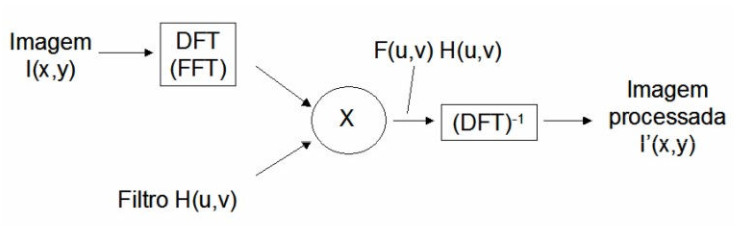
\includegraphics[width=0.7\textwidth]{template/img/fig.png}
        \caption{Esquema ilustrando os passos da filtragem no domínio da frequência.}
        \label{fig:fig}
    \end{figure}
    
    A transformada de Fourier pode ser utilizado na forma unidimensional ou bidimensional. Na transformada de Fourier os dados não são perdidos na transformação, eles apenas estão sendo representados de uma outra forma.
    
    Para Aconci\footnote{\url{http://www2.ic.uff.br/~aconci/filtragemdominiofrequencia.pdf}}, a princípio parece difícil entender a visualização da imagem, pois, um ponto de uma imagem  representada  no  domínio  Fourier  (ou  da  frequência)  pode  conter  informações  sobre toda  a  imagem  no  domínio  espacial  (figura  10),  indicando  quanto  desta  frequência  há  na  imagem.
    
     \begin{figure}[H]
        \centering
        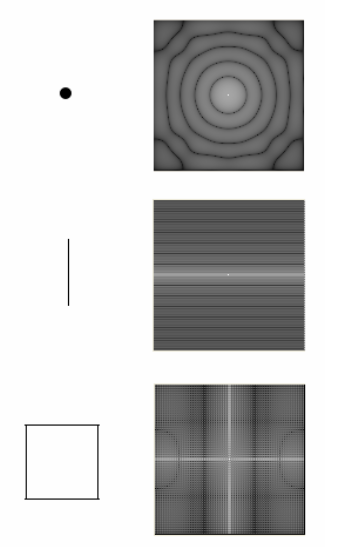
\includegraphics[width=0.6\textwidth]{template/img/fig10.png}
        \caption{Algumas funções bidimensionais e seus aspectos de Fourier.}
        \label{fig:fig10}
    \end{figure}
    
    \subsection{Transformada de Fourier Unidimensional}
    De acordo com \citeonline{adair}, a transformada de Fourier de uma função contínua f(x) de uma variável real x pode ser definida como:
    
     \begin{figure}[H]
        \centering
        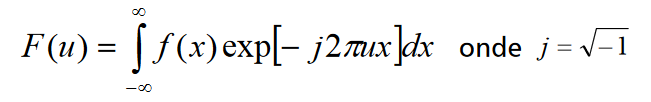
\includegraphics[width=0.6\textwidth]{template/img/fig11.png}
        \caption{Função contínua de uma variável real x.}
        \label{fig:fig11}
    \end{figure}
    
    A partir de F(u), pode-se obter f(x) através da transformada inversa de Fourier:
    
     \begin{figure}[H]
        \centering
        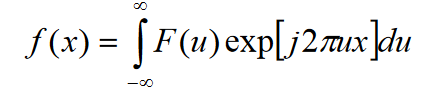
\includegraphics[width=0.4\textwidth]{template/img/fig12.png}
        \caption{Transformada inversa de Fourier.}
        \label{fig:fig12}
    \end{figure}
    
    As  duas  equações  são  chamadas  de  par  de transformada de Fourier e podem existir se forem integráveis e se f(x) for contínua.
    
    A transformada de Fourier de uma função é uma função complexa:
    
    \begin{figure}[H]
        \centering
        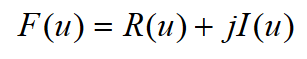
\includegraphics[width=0.3\textwidth]{template/img/fig13.png}
        \caption{Função transformada de Fourier.}
        \label{fig:fig13}
    \end{figure}
    
    que pode ser descrita na forma: 
    
    \begin{figure}[H]
        \centering
        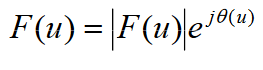
\includegraphics[width=0.3\textwidth]{template/img/fig14.png}
        \caption{Função transformada de Fourier detalhada.}
        \label{fig:fig14}
    \end{figure}
    
    onde: 
    
     \begin{figure}[H]
        \centering
        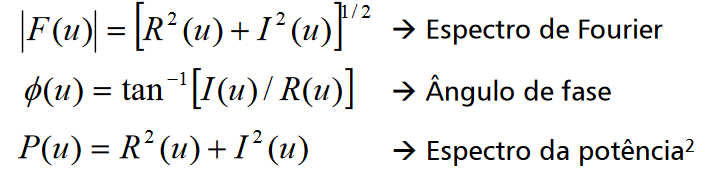
\includegraphics[width=0.7\textwidth]{template/img/fig15.png}
        \caption{Explicação dos termos.}
        \label{fig:fig15}
    \end{figure}
    
    \subsection{Transformada de Fourier Bidimensional}
    
    De acordo com \citeonline{adair}, a transformada de Fourier para uma função bidimensional, pode ser descrita como:
    
    \begin{figure}[H]
        \centering
        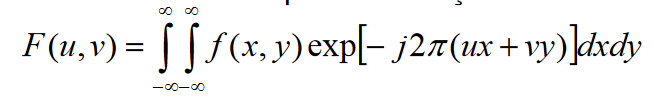
\includegraphics[width=0.6\textwidth]{template/img/fig16.png}
        \caption{Função bidimensional Fourier.}
        \label{fig:fig16}
    \end{figure}
    
    Sendo que a sua função inversa é descrita da seguinte forma:
    
     \begin{figure}[H]
        \centering
        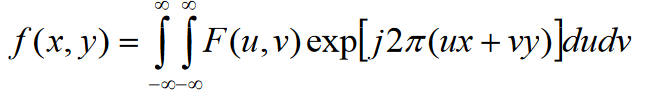
\includegraphics[width=0.6\textwidth]{template/img/fig17.png}
        \caption{Função bidimensional Fourier inversa.}
        \label{fig:fig17}
    \end{figure}
    
    onde:
    
    \begin{figure}[H]
        \centering
        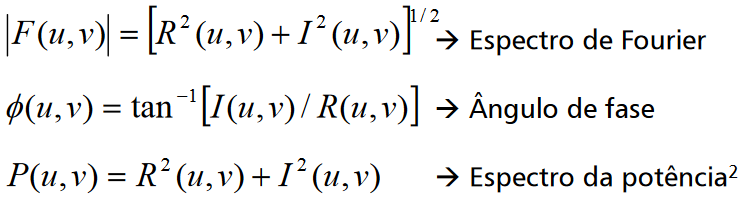
\includegraphics[width=0.8\textwidth]{template/img/fig18.png}
        \caption{Explicação detalhada da função bidimensional.}
        \label{fig:fig18}
    \end{figure}
    
    \section{Conclusão}
    Neste documento foi feita uma breve introdução a visão computacional, explicando alguns termos de processamento de imagens que podem ser utilizados nesta matéria. Caso deseje ampliar mais o seu conhecimento sobre o assunto, visite as aulas citadas na referencia deste documento.

\medskip

% References
\small
\bibliographystyle{abntex2-alf}
\bibliography{bibliography}
\end{document}
